%!TEX root = ../thesis.tex

\cleardoublepage
\chapter{Approach}
\label{cha:approach}


This chapter covers how the problem was addressed and how the proposed solution was integrated into a scientific workflow manager and tested. This chapter will first look over the software architecture of the approach and where it was inserted into the source code of nextflow, then the exact nature of the gradient bandit and the Q-learning approaches will be considered. Finally the structure of the tests performed to try and evaluate these approaches will explained before the results from those tests are presented and discussed in the next chapter. 

%%=========================================
\section{Integrating a Solution into a Workflow Manager}
\label{sec:integration}

Nextflow is a very robust scientific  workflow management system written primarily in groovy. It supports various execution platforms and has a large variety of tools to help users analyse the performance of their workflows \cite{TracingAndVisualisation}. Nextflow is free open source software and for this thesis a fork of the 20.12.0 version was used. In order to integrate a reinforcement learning approach with the nextflow source code a simple structure was designed which externalised the storage of the data of previous tasks and workflow runs to a database and when a task needed to be scheduled, the reinforcement learning agent would use the historical data for that task to inform its decision. The structure can be seen in the following figure.

\begin{figure}[ht]
    \centering
        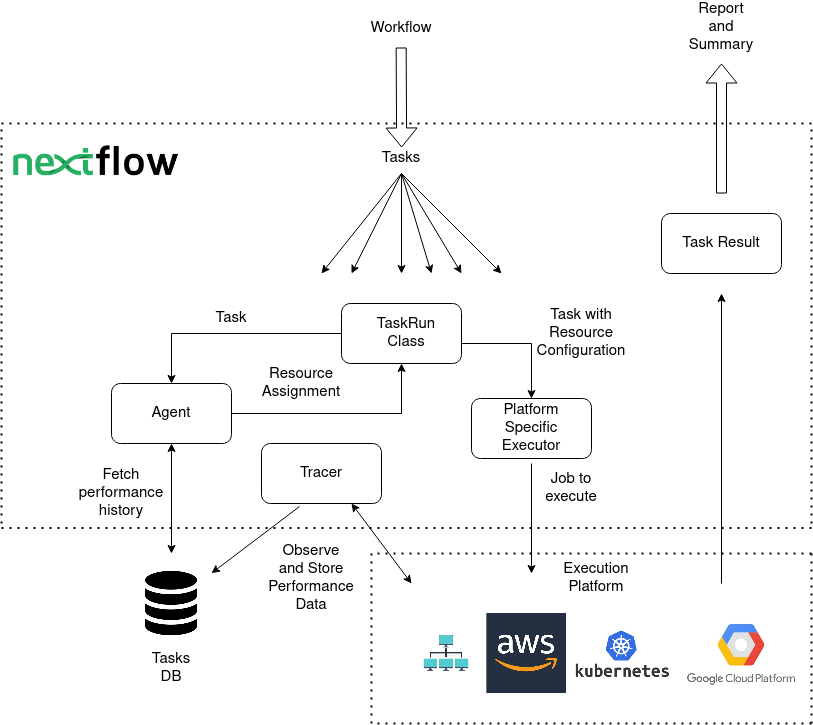
\includegraphics[width=0.8\textwidth]{fig/implementation_diagram.png}
        \caption{High Level Design: Integration of a Reinforcement-Learning Agent into Nextflow}
        \label{fig:implementation}
\end{figure}

Before a task is ready to be scheduled it is first sent to the reinforcement-learning agent specific to that task. For the purposes of this thesis that was either a Q-learning agent or a gradient bandit. The task’s agent would then select historical performance data and any other relevant data (i.e. what state the agent was last in) from the database. This database is external to nextflow and the creation and management of this database is not performed by nextflow or the agent- nextflow and the agent only use the database to save or read data between workflows. Using this data, the agent selects a new resource allocation for the task and overwrites the task’s default configuration. After this nextflow uses its custom executor for the given execution platform to prepare the task and pass it on to that platform. The task is then executed. It is important to note that the execution platform will also have its own system for managing, scheduling and executing jobs and processes but from the perspective of the nextflow/agent system all it does is pass on the task with the resource allocations which were chosen. As the task is executed nextflow’s tracer module will gather performance data, i.e. peak CPU usage, peak RSS and other such things \cite{TracingAndVisualisation}. Once the task is finished all of this data is stored in the  database to be used by the agent the next time the task comes. It is important to note that there is one agent for each unique task. These agents are called whenever their task needs to be executed and they use the database to receive rewards for their previous actions.


Now that the structure of the agent’s environment has been explained and the relationship between task scheduling and collecting data about a task is clear, it is time to delve into the specific approaches tried.

\section{CPU Bandit}
\label{sec:cpu_bandit}

\subsection{Design}
\label{sub:bandit1_design}

The first bandit or CPU Bandit, as it was nicknamed, had a very simple set of actions to choose from which were based on the number of CPUs available to the system. The bandit then learned how many CPUs to allocate to the task. Its reward was based on a very straightforward function:

\begin{equation}\label{bandit1_reward}
reward = -t\times(1+cpus - cpu\_usage/100)
\end{equation}


In this equation $cpu\_usage$ is a value in percent of the number of single core CPUs used by the task. If a task were assigned 4 CPUs and only effectively used two of them then $cpu\_usage$ would be $200$\%. $cpus$ is the number of CPUs assigned to the task and $t$ is how long the task took to run. Put in other words this equation punishes the agent with a negative reward equal to the amount of time it ran plus the unused CPU time (time multiplied by the number of unused CPUs). The idea is that the agent is incentivised to try to minimise the amount of time where any of the allocated CPU’s are not being used, and by punishing it with the amount of time that the task ran for the agent is also encouraged to try to reduce the amount of time taken for the task to complete. Additionally, should a task have 100\% usage then its penalty is not 0 but is just the time that it ran. The reason for this is that if the agent has no concept of time it will always allocate the least amount of resources possible, since that immediately minimises the amount of resources wasted, and ultimately the tasks and their workflows would be incredibly slow. 

\subsection{Picking the Right Step Size}
\label{sub:const_stepsize}
One immediate issue encountered with the CPU bandit was related to the step size. The initial step size $\alpha$ was $0.1$ which would be an appropriate step size for a bounded reward function with a maximum less than 20 or a function which is known to have a standard deviation less than that. However the reward function used in \ref{bandit1_reward} has the bounds [ $-time*(cpus+1)$ , $-time$ ] and as such is effectively unbounded since time can be arbitrarily large (all tasks are of course configured with a maximum runtime but these are user estimates and are always several orders of magnitude larger than the normal time it takes, e.g. maximum runtime is usually an order of days whereas the maximum runtime seen for any task in the course of these experiments was an order of minutes). Additionally over the course of the experiments in this thesis the standard deviation which was observed for the reward function was usually too large for this step size as well.  The danger in using an inappropriate constant step size for a given reward function is that when the bandit receives a reward which is larger or smaller than the previous average, the step taken in the direction of that action will be too large and the bandits preferences will be updated such that the given action is always preferred and no other actions are tried any more. This causes the bandit to cease with the exploration phase too early. This effect was most commonly occurring for tasks which took longer than 20 seconds to complete and was especially pronounced for tasks with runtimes of 100 seconds and more.  For these tasks the inherent volatility of the reward function (volatile relative to a step size of 0.1) meant that the bandits were converging very early and often had not explored the other actions at all. For example if one allocation receives a reward of -150 and and the first two allocations had had an average reward of 350 then for a step size of 0.1 the preference for the new allocation will increase by 5. Because of the exponential nature of the soft max distribution function used on the preferences this increase could result in the bandit converging to always pick the third allocation without any more exploration. 

% \begin{figure}[ht]
    %\centering
       % 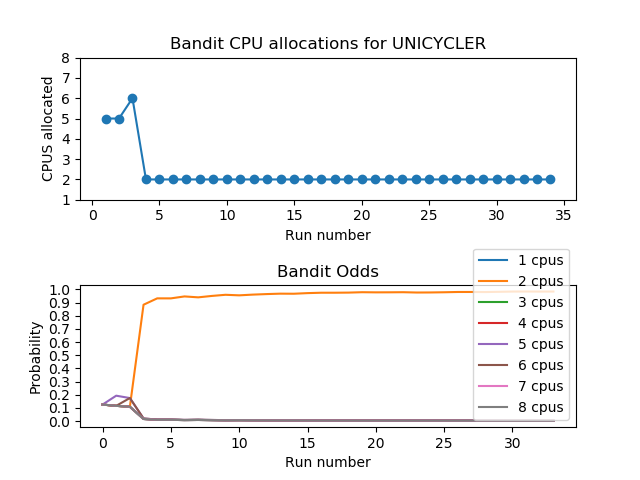
\includegraphics[width=0.8\textwidth]{fig/old_UNICYCLER.png}
        %\caption{Example of Bandit Converging Too Early}
        %\label{fig:old_unicycler}
%\end{figure}

\begin{figure}[ht]
\centering
\begin{subfigure}{.5\textwidth}
  %\centering
  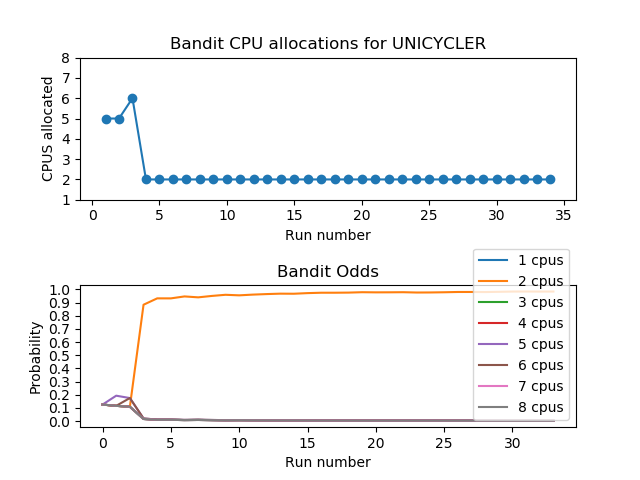
\includegraphics[width=1.1\textwidth,height=1.1\textwidth]{fig/old_UNICYCLER.png}
  \caption{Bandit 1}
  %\label{fig:sub1}
\end{subfigure}%
\begin{subfigure}{.5\textwidth}
 % \centering
  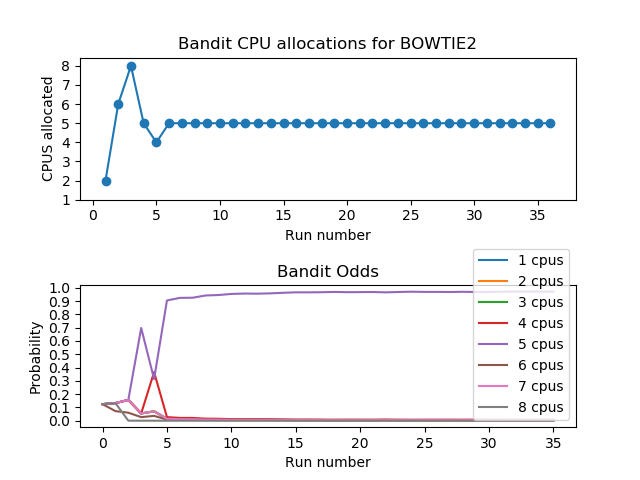
\includegraphics[width=1.1\textwidth,height=1.1\textwidth]{fig/old_BOWTIE2.png}
  \caption{Bandit 2}
  %\label{fig:sub2}
\end{subfigure}
\caption{Example of Two Bandits Converging Too Fast}
\label{fig:old_bandits}
\end{figure}

These two examples are of two tasks which were exhibiting the behaviour described previously. The figures display the action chosen by the bandit in the top graph and the probabilities for all of the actions in the bottom graph. As can be seen the probability for a given action rises far too quickly and no other actions are attempted. This is occurring because the step taken by the bandit in the direction of a single actions preference is too large and the resulting probability for that action (probability of choosing a given action is based on a soft max distribution of the preferences for the available actions) grows too fast so that only that action is being chosen. 

The solution to this problem is to adjust the step size so that it is not a constant value but is instead based on the average time (historically) that it takes the task to complete. So tasks which have longer average runtimes are given smaller step sizes. The reference equation used was $step\_size = 1/max(reward)$, which for the reward function in \ref{bandit1_reward} translated to $step\_size = 1/avg(time)$ since the maximum possible absolute value of the reward would be close to $cpus*avg\_time$. This reference equation is based on the Gradient Bandit example in the Sutton and Barto book, where they used a step size of 0.1 for a reward function which had a statistical mean of 4.  

\begin{figure}[ht]
\centering
\begin{subfigure}{.5\textwidth}
  %\centering
  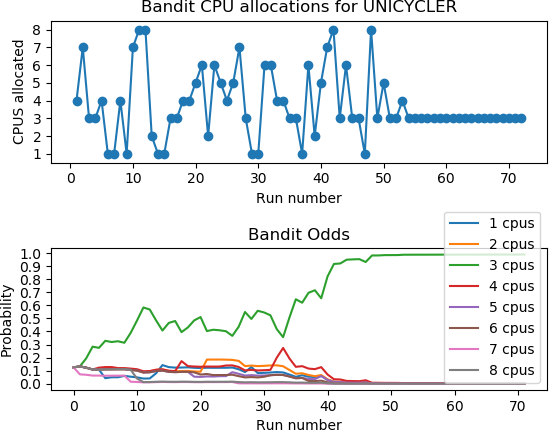
\includegraphics[width=1.1\textwidth,height=1.1\textwidth]{fig/UNICYCLER.png}
  \caption{Bandit 1}
  %\label{fig:sub1}
\end{subfigure}%
\begin{subfigure}{.5\textwidth}
 % \centering
  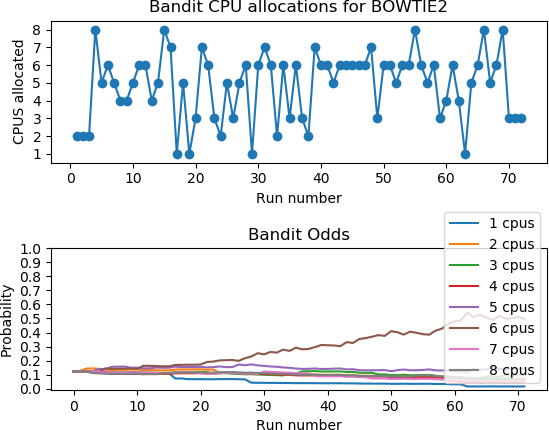
\includegraphics[width=1.1\textwidth,height=1.1\textwidth]{fig/BOWTIE2.png}
  \caption{Bandit 2}
  %\label{fig:sub2}
\end{subfigure}
\caption{Bandits with a Step Size Based on Their Historical Average Execution Time}
\label{fig:fixed_bandits}
\end{figure}

The above figure shows the same two tasks and their bandits but with the changes to the step size. As can be seen the exploration phase is considerably longer and many different CPU allocations (actions) are tried before settling on one. Specifically in the case of the \textit{UNICYCLER} task’s bandit we can see that although allocating 3 CPUs seems to develop a strong preference early on (perhaps because it performed abnormally well once or perhaps because it genuinely is the best possible allocation) it does not become so preferred as to be dominant until much later and the bandit continues trying other options as well.

It should be noted however that these changes mean that for optimal performance of the bandits there should already be amount of historical data about the task’s and their runtimes available. It is not a necessity because over time the bandit can gather this data itself, but it is preferable.  Since some reference data is needed to compare to the bandits, in order to evaluate their performance, it makes sense to first collect the reference data about the performance of the default configurations and then run the workflows with the bandits active.

\section{Q-Agent}
\label{sec:q_agent}

Similar to the approach with the gradient bandits, there was one Q-learning agent per unique task. The Q-learning agent’s state was always the current allocation of cpu and memory for the given task, and as its set of actions it could choose between incrementing or decrementing the amount of cpus or memory, or it could do nothing. To limit the state space the maximum and minimum number of cpus and memory as well as the amount by which they were incremented or decremented was based first on the maximum resources of the system and secondly on the default allocation given to the task by the developers of the workflow. When the task was scheduled by the agent for the first time it would start in the default state.

The pseudo code for the Q-learning agent can be seen in \ref{alg:q-learning}.

\begin{algorithm}[H]
Initialise $Q(s,a) = 0$\\
Initialise start state $s$\\
\While{\textbf{True}}{
        \eIf{$random < \epsilon$}{choose random action $a$}{choose action $a = max_a (Q(s,a))$}
        Take action $a$, receive reward $r$, transition to state $\hat{s}$\\
        Update $Q_{new}(s,a) = Q(s,a) + \alpha \times (r + \gamma \times max_{\hat{a}}(Q(\hat{s},\hat{a})) - Q(s,a) )$\\
}
\caption{Q-learning Agent Pseudocode}
\label{alg:q-learning}
\end{algorithm}


For the Q-Agent a different reward function was used than for the gradient bandit- primarily because it also had to incorporate memory but also as part of an attempt to try slightly different reward functions and approaches. 

\begin{equation}\label{q_agent_1_reward}
r = -max(0.1,cpus-cpu\_usage/100) \times (t/avg\_t) \times (mem\times (1 - max(0.75,mem\_usage/100)))
\end{equation}

Here the $memory$ variable refers to the memory allocated to the process and $mem\_usage$ is the value of of the peak RSS of the process divided by the memory assigned to it. $avg\_t$ is a constant value which is determined at runtime based on the historical average execution time for the task. Since division by the task’s average time is incorporated into the reward function it did not need to be incorporated into the step size as with the gradient bandit and the issues associated with that were avoided. This function is effectively a product of the number of unused CPUs, the slow-down factor and the amount of unused memory. There are some slight modifications though. The $max$ function is used to set an artificial floor for the penalty incurred by the unused CPUs and unused memory. Tasks which use more than 90\% of the available CPUs are given the same reward as tasks which use exactly 90\% in an attempt to prevent the agent from deciding to assign each task 1 CPU in order to minimise the amount of unused CPUs. Additionally the floor for unused memory is capped at 25\% in a similar manner. This is done to discourage the agent from allocating too little memory because tasks which use too much memory will of course be killed and have to start over, which has a hugely detrimental effect on performance. This reward function is of course negated in order to turn it into a penalty function so that the agent will seek to minimise its penalty by minimising the unused CPUs, slowdown and unused memory.

The Q-learning agent also has 3 other parameters- the step size $\alpha$, epsilon $\epsilon$ and the discount $\gamma$. Step size was set to 0.1 and the discount was 1.0. Epsilon is adjusted over time- at first it is 0.5, to encourage exploration, then after 50 runs it is decreased to 0.25 and after 100 runs it is 0.1 to discourage exploration but leave room for the bandit to still occasionally try other actions and wind up in different states.

\section{Testing the Agents}
\label{sec:testing}

In order to evaluate the performance of these agents they were tested on a 34-core, 128GB RAM machine against 5 different workflows. Each workflow is run 10 times without any reinforcement learning agents active. This was done to have something to compare the results to later but also so that there was historical data about the average time each of the tasks take since the reinforcement learning agents need this information. After that the agents are tested. The gradient bandits are run 50 times for each workflow and the Q-learning agents 100 times.

The input data used for the workflows is based on custom combinations of different input files provided by the workflow's maintainers- there are the full example datasets and the short example datasets. The combinations are designed to strike a balance between having large input data and realistic task configurations but also being short enough that it is feasible to run the workflows hundreds of times. For reference, the full datasets will often take 6 hours or more to run once whereas the short examples never take more than 5 minutes. 

The nextflow source code inherently keeps track of the total number of resources available and the resources already assigned to tasks and it will not schedule more resources than the system has. The tasks are all run inside of docker containers with exactly number of CPUs and memory requested by the task. 

For the final comparison in the evaluation chapter the 10 runs without the agents were compared to the last 10 runs with each of the agents.


